\lab{Applications}{Image Segmentation}{Image Segmentation}

\objective{Understand some basic applications of Eigenvalues to graph theory}
\label{lab:ImgSeg_eigenvalues}

A graph is a mathematical construct used to encode how things are connected. Let us briefly review the basic terminology.
Recall that a graph is defined as a collection of vertices, which can be thought of as different destinations, and edges, which can be thought of as roads connecting destinations together.
Figure \ref{segmentation:graph} is a simple example of a graph.

\begin{figure}
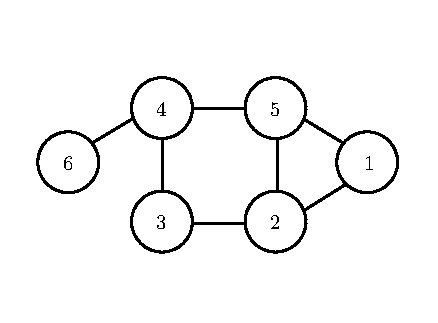
\includegraphics[scale=0.4]{graphExample}
\caption{A simple graph.}
\label{segmentation:graph}
\end{figure}

In that example, we have a collection of six vertices and seven edges.
We denote the number of vertices in a graph by $|V|$, and the number of edges by $|E|$.
The edges can carry direction information (directed graphs) or they can be bidirectional (undirected graphs, like the example).
One way to encode all the information in this picture is to use what is called an adjacency matrix.

\begin{definition} An adjacency matrix $A$ is a $|V| \times |V|$ matrix where the $(i,j)$-th entry $a_{ij}$ is
\begin{center}
	$a_{ij} = \begin{cases} 1 & \mbox{If an edge connects vertex i to vertex j} \\ 0 & \mbox{otherwise} \end{cases}$
\end{center}
%technically, the definition does not apply to all graphs (according to Wikipedia)
%however, this definition works if we are just considering simple graphs, i.e. at most one edge between any two vertices, no loops
\end{definition}

So for the graph in Figure \ref{segmentation:graph}, we have the following adjacency matrix:
\[
\begin{pmatrix}
0 & 1 & 0 & 0 & 1 & 0 \\
1 & 0 & 1 & 0 & 1 & 0 \\
0 & 1 & 0 & 1 & 0 & 0 \\
0 & 0 & 1 & 0 & 1 & 1 \\
1 & 1 & 0 & 1 & 0 & 0 \\
0 & 0 & 0 & 1 & 0 & 0 \\
\end{pmatrix}
\]

Note that the adjacency matrix of an undirected graph is symmetric.
We may also define weighted graphs so that each edge has a weight or cost attached to it.
In this case the adjacency matrix will have the cost in each entry, rather than just a 1 or 0.
An example of a weighted may be a collection of cities as vertices, roads connecting them as edges, and the distance of the connecting roads as the cost attached to each edge.

In this lab we will be investigating the sorts of things that we can discover about a graph by examining the spectrum of its adjacency matrix.
While the formulation of the adjacency matrix seems to be very simple, its structure allows us to learn surprising things by examining its eigenvalues.

We begin by first looking at the definition of the Laplacian of a graph:

\begin{definition}  The \emph{degree} of a vertex of a weighted graph is the sum of the weights of the edges connected to that vertex.
In undirected graphs, which is what we will be dealing with, this is the sum of all the weights moving into that vertex.
This definition varies slightly for directed graphs.
Let $D$ be a diagonal matrix with
\[
D_{ii} = \mbox{ Degree of vertex $i$}
\]
and let $A$ be the adjacency matrix of the graph.
The graph \emph{Laplacian} $Q$ is given by
\[
Q = D-A
\]
\end{definition}

The Laplacian matrix of a graph will typically be very sparse.
We will be examining the spectrum of the Laplacian matrix.

A connected graph is a graph where every vertex is connected to every other vertex by at least one path.
An important question one might ask about a graph is whether or not it is connected.
What is the best way to do this?
A naive approach would be to exhaustively map every possible path from each vertex.
While this would be feasible for very small graphs, most interesting graphs (for example, the internet) will have thousands of vertices and such an approach becomes essentially impossible to execute.

It turns out there is a better way.
If the second smallest eigenvalue of the Laplacian matrix associated with a graph is positive, then this graph is connected.
The mathematics behind this is quite involved, so we omit a proof for now.
In many applications the Laplacian matrix will be very sparse, and thus with optimizations made for sparsity, we can discover the connectivity of a graph relatively cheaply.

\begin{problem}Write a function \li{laplacian} that accepts an adjacency matrix as an argument and returns the Laplacian matrix and its second smallest eigenvalue.
Use the \li{scipy.linalg} package to compute this eigenvalue.
Using {\tt numpy.rand(n,n)}, generate several random matrices of various sizes.
Use masking to change the sparsity of said matrices, i.e. {\tt numpy.rand(n,n) > c} for {\tt c = 0.25,0.5,0.75}.
Try different distributions and $c$ values.
What can we expect about the connectivity of random matrices?
\end{problem}

A related problem is found in image processing.
An image is a collection of coordinates and light intensities.
We call each coordinate and associated brightness a pixel.
We let every pixel in an image be a vertex in a graph that is connected to its neighbors within a certain radius.
For an $N \times N$ image, we define an adjacency matrix as follows:

\begin{equation}
\label{eq:adjacency}
w_{ij} = e^{-\frac{|I(i) - I(j)|}{\sigma_I^2}} \cdot \begin{cases} e^{-\frac{d(i,j)}{\sigma_d^2}} & \mbox{ for $d(i,j) < r$} \\ 0 & \mbox{ otherwise} \end{cases}
\end{equation}
for $i = 1 \hdots N^2$ and $j = 1 \hdots N^2$ (traveling through each pixel in the image), where
\begin{itemize}
	\item$d(i,j)$ is the Euclidean distance between pixel $i$ and pixel $j$
	\item $|I(i) - I(j)|$ is the difference in brightness of pixels $i$ and $j$
	\item $\sigma_I$ and $\sigma_d$ are constants
\end{itemize}
Thus, given a $N\times N$ image, we will produce an adjacency matrix of size $N^2\times N^2$.
Even for smaller images, this will become very large, but we have sparsity on our side.
Even so, only do this for images smaller than 50 by 50.
Since each pixel is only connected to the pixels within radius $r$ around it, relatively few entries will be non-zero.

\begin{problem}
Write a function \li{adjacency} that takes an $N \times N$ image array, radius $r$, and values for
$\sigma_I^2$ and $\sigma_d^2$, and returns the adjacency matrix defined in \eqref{eq:adjacency}.
Notice that for each pixel you can save time by only checking the pixels $r$ rows and columns away.
%For that you'll have to handle the pixels on the edges and corners of the image carefully.
%I gave them new helper code, which abstracts away the edge cases.
Make use of sparsity in order to feasibly store such a large matrix.
We have provided code to help out with this problem.
\end{problem}

An important problem in image processing is that of image segmentation.
When humans observe an image, they can easily pick out portions of an image that ``belong together.''
For example, if we saw the picture of a person against a black background, the pixels making up the background would make up one segment of an image, and the person would make up the other part.
While this seems simple for a human, how can we program a computer to do so?

Once again, we turn to the eigenvalues of the Laplacian matrix.
We examine the second smallest eigenvalue of $D^{-\frac{1}{2}}QD^{-\frac{1}{2}}$, where $D$ is the degree matrix and $Q$ is the Laplacian matrix of the adjacency matrix defined in \eqref{eq:adjacency}.
The associated $N^2 \times 1$ eigenvector will have positive and negative entries, splitting the image into two parts.
Thanks to some very fancy mathematics and the way we have defined the weights between nodes, this does a pretty good job of breaking an image into two segments.
Recursively executing this function, we can find segments within segments.
%Figure \ref{segmentation:example} shows a simple example of an image and its segments.

%\begin{figure}
%\includegraphics[scale=0.2]{monument}
%\includegraphics[scale=0.2]{segment1}
%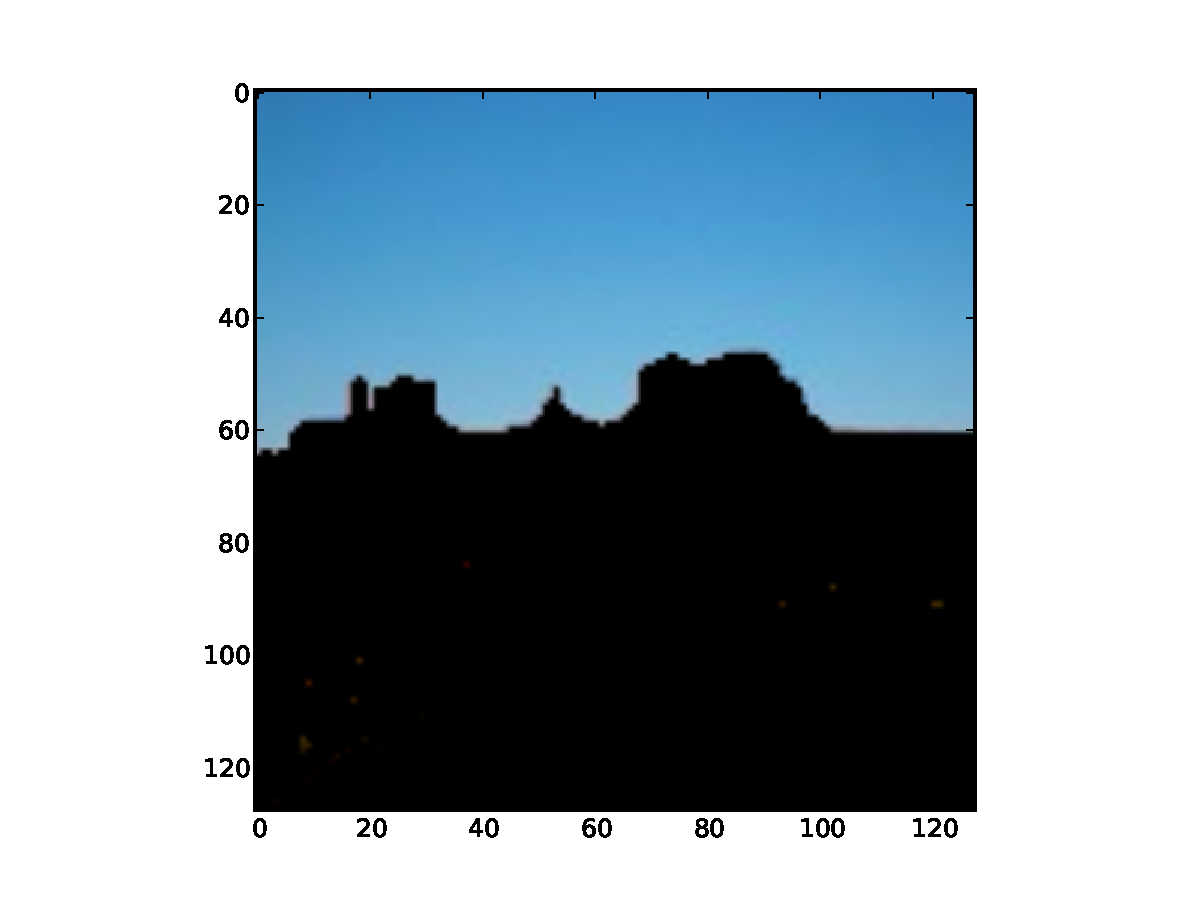
\includegraphics[scale=0.2]{segment2}
%\caption{An image and it's segments.}
%\label{segmentation:example}
%\end{figure}

\begin{problem}  Write a function \li{segment} that solves the segmentation problem for small images.
Accept an image array as an argument and return the two segments.
Use $r = 5, \sigma_I^2 = 0.02,$ and $\sigma_d^2 = 3.0$.
Remember that the Laplacian matrix will be very large but also very sparse.
Because of the way we defined $\sigma_I^2$ the image matrix intensity values need to be between $0.0$ and $1.0$.
\end{problem}
